% !TEX program = xelatex
\documentclass[11pt,fontset=none]{ctexart}

\usepackage[a4paper,left=18mm,right=18mm,top=18mm,bottom=18mm]{geometry}
\usepackage{fontspec}
\usepackage{graphicx}
\usepackage[table]{xcolor}
\usepackage{array,tabularx,booktabs,multirow}
\usepackage{tikz}
\usetikzlibrary{arrows.meta,positioning,fit,calc,backgrounds,shapes.geometric,shadows.blur}
\usepackage{tcolorbox}
\tcbuselibrary{skins,breakable}
\usepackage{titlesec}
\usepackage{enumitem}
\usepackage{fancyhdr}
\usepackage{setspace}
\usepackage{amsmath}
\usepackage{hyperref}
\usepackage{xurl}
\usepackage{caption}
\usepackage{ragged2e}
\usepackage{pifont}
\hypersetup{colorlinks=true,linkcolor=black,urlcolor=black}

% ---------- Fonts ----------
\defaultfontfeatures{Ligatures=TeX,Scale=MatchLowercase}
\setmainfont{Baskerville}
\setsansfont{Avenir Next}
\setmonofont{Menlo}
\setCJKmainfont[
  BoldFont={Songti SC Bold},
  ItalicFont={Songti SC},
  BoldItalicFont={Songti SC Bold}
]{Songti SC}
\setCJKsansfont[
  BoldFont={Hiragino Sans GB W6},
  ItalicFont={Hiragino Sans GB W3},
  BoldItalicFont={Hiragino Sans GB W6}
]{Hiragino Sans GB W3}
\setCJKmonofont[
  BoldFont={Hiragino Sans GB W6},
  ItalicFont={Hiragino Sans GB W3},
  BoldItalicFont={Hiragino Sans GB W6}
]{Hiragino Sans GB W3}
\newCJKfontfamily\titlecjk[
  BoldFont={Lantinghei SC},
  ItalicFont={Lantinghei SC},
  BoldItalicFont={Lantinghei SC}
]{Lantinghei SC}

% ---------- Colors ----------
\definecolor{MiraInk}{HTML}{2D2A2C}
\definecolor{MiraGray}{HTML}{6F6667}
\definecolor{MiraLine}{HTML}{D9D0CD}
\definecolor{MiraBg}{HTML}{F8F4F1}
\definecolor{MiraSoft}{HTML}{F3ECE8}
\definecolor{MiraRose}{HTML}{EFE3DE}
\definecolor{MiraAccent}{HTML}{7C4A53}
\definecolor{MiraAccent2}{HTML}{B77B62}
\definecolor{MiraGreen}{HTML}{43695A}
\definecolor{MiraGreenSoft}{HTML}{EDF4F0}
\definecolor{MiraBlue}{HTML}{4E6A93}
\definecolor{MiraBlueSoft}{HTML}{EDF2FA}
\definecolor{MiraGold}{HTML}{B58A58}
\definecolor{MiraGoldSoft}{HTML}{FBF4E9}
\definecolor{MiraWarn}{HTML}{8F3E2D}
\definecolor{MiraWarnSoft}{HTML}{FBEEEA}

% ---------- Global layout ----------
\setlength{\parindent}{0pt}
\setlength{\parskip}{0.35em}
\setstretch{1.15}
\renewcommand{\arraystretch}{1.22}
\pagestyle{fancy}
\fancyhf{}
\lhead{\footnotesize\sffamily\color{MiraGray} MIRA｜项目说明书}
\rhead{\footnotesize\sffamily\color{MiraGray} OpenClaw Hackathon}
\cfoot{\footnotesize\sffamily\color{MiraGray}\thepage}
\renewcommand{\headrulewidth}{0pt}

\titleformat{\section}
  {\Large\bfseries\sffamily\titlecjk\color{MiraInk}}
  {\thesection.}{0.55em}{}
\titlespacing*{\section}{0pt}{0.1em}{0.45em}

\titleformat{\subsection}
  {\normalsize\bfseries\sffamily\titlecjk\color{MiraInk}}
  {}{0pt}{}
\titlespacing*{\subsection}{0pt}{0.5em}{0.25em}

\newcolumntype{Y}{>{\RaggedRight\arraybackslash}X}
\newcolumntype{C}[1]{>{\Centering\arraybackslash}p{#1}}
\newcolumntype{L}[1]{>{\RaggedRight\arraybackslash}p{#1}}

\setlist[itemize]{leftmargin=1.35em,itemsep=0.25em,topsep=0.25em,parsep=0em,partopsep=0em}

\newtcolorbox{card}[2][]{
  enhanced,
  breakable,
  colback=white,
  colframe=MiraLine,
  boxrule=0.9pt,
  arc=4pt,
  left=10pt,right=10pt,top=8pt,bottom=8pt,
  title={#2},
  colbacktitle=MiraSoft,
  coltitle=MiraInk,
  fonttitle=\bfseries\sffamily\titlecjk,
  #1
}

\newtcolorbox{accentcard}[2][]{
  enhanced,
  breakable,
  colback=MiraRose,
  colframe=MiraAccent,
  boxrule=0.9pt,
  arc=4pt,
  left=10pt,right=10pt,top=8pt,bottom=8pt,
  title={#2},
  colbacktitle=MiraAccent,
  coltitle=white,
  fonttitle=\bfseries\sffamily\titlecjk,
  #1
}

\newtcolorbox{greencard}[2][]{
  enhanced,
  breakable,
  colback=MiraGreenSoft,
  colframe=MiraGreen,
  boxrule=0.9pt,
  arc=4pt,
  left=10pt,right=10pt,top=8pt,bottom=8pt,
  title={#2},
  colbacktitle=MiraGreen,
  coltitle=white,
  fonttitle=\bfseries\sffamily\titlecjk,
  #1
}

\newtcolorbox{bluecard}[2][]{
  enhanced,
  breakable,
  colback=MiraBlueSoft,
  colframe=MiraBlue,
  boxrule=0.9pt,
  arc=4pt,
  left=10pt,right=10pt,top=8pt,bottom=8pt,
  title={#2},
  colbacktitle=MiraBlue,
  coltitle=white,
  fonttitle=\bfseries\sffamily\titlecjk,
  #1
}

\newtcolorbox{goldcard}[2][]{
  enhanced,
  breakable,
  colback=MiraGoldSoft,
  colframe=MiraGold,
  boxrule=0.9pt,
  arc=4pt,
  left=10pt,right=10pt,top=8pt,bottom=8pt,
  title={#2},
  colbacktitle=MiraGold,
  coltitle=white,
  fonttitle=\bfseries\sffamily\titlecjk,
  #1
}

\newcommand{\goodtag}[1]{\tikz[baseline=(n.base)]\node[rounded corners=2pt,fill=MiraGreenSoft,draw=MiraGreen,inner xsep=4pt,inner ysep=2pt](n){\footnotesize\sffamily\color{MiraGreen} #1};}
\newcommand{\midtag}[1]{\tikz[baseline=(n.base)]\node[rounded corners=2pt,fill=MiraBlueSoft,draw=MiraBlue,inner xsep=4pt,inner ysep=2pt](n){\footnotesize\sffamily\color{MiraBlue} #1};}
\newcommand{\futuretag}[1]{\tikz[baseline=(n.base)]\node[rounded corners=2pt,fill=MiraGoldSoft,draw=MiraGold,inner xsep=4pt,inner ysep=2pt](n){\footnotesize\sffamily\color{MiraGold} #1};}

\begin{document}

% ================= Cover =================
\thispagestyle{empty}
\begin{tikzpicture}[remember picture,overlay]
  \fill[MiraBg] (current page.south west) rectangle (current page.north east);
\end{tikzpicture}
\vspace*{-18mm}
\noindent
\includegraphics[width=\paperwidth]{assets/cover-banner.png}

\vspace{8mm}
{\Huge\bfseries\sffamily\titlecjk\color{MiraInk} Mira 项目说明书\par}
\vspace{1mm}
{\large\sffamily\color{MiraAccent} 有些关心，不需要开口\par}
\vspace{3mm}
{\normalsize\color{MiraGray} A proactive, low-disturbance AI companion built around real-time sensing, memory, judgment and action.\par}

\vspace{7mm}
\begin{card}{一句话领起}
Mira 不是一个等待用户提问的聊天框，而是一套\textbf{“先感知、再判断、后行动”}的陪伴系统：它借助\textbf{AR 眼镜、可穿戴信号、环境上下文与智能家居执行面}，在你最不愿开口、也最需要被照顾的时刻，给出\textbf{克制、私密、可解释}的支持。
\end{card}

\vspace{3mm}
\begin{tabularx}{\linewidth}{|Y|Y|Y|Y|}
\hline
\rowcolor{MiraSoft}
\centering\textbf{Perception} & \centering\textbf{Memory} & \centering\textbf{Judgment} & \centering\textbf{Action}\tabularnewline
\hline
\centering 眼镜画面、心率、环境线索 & \centering 短期状态与长期偏好记忆 & \centering 先判断“值不值得打扰” & \centering 镜片提示、耳机/手表、家居执行\tabularnewline
\hline
\end{tabularx}

\vfill
\begin{tabularx}{\linewidth}{Y Y}
\textcolor{MiraGray}{\footnotesize\sffamily 赛道定位}\par
{\bfseries 生活龙虾｜把日子过好}
&
\textcolor{MiraGray}{\footnotesize\sffamily 文档用途}\par
{\bfseries 面向评委与合作伙伴的正式项目说明}
\end{tabularx}
\newpage

% ================= Page 2 =================
\section*{领起与目录}
\begin{accentcard}{这份说明书想回答的不是“它酷不酷”，而是“它能不能真正照顾人”}
今天大量所谓的陪伴式 AI，仍然停留在“\textbf{你说，它答}”的范式里；而真正需要帮助的时刻，往往发生在用户\textbf{无暇表达、甚至不愿表达}的那几分钟。Mira 的出发点，就是把这段交互空白补上：让系统在被允许的边界内更早一点察觉，更稳一点行动。
\end{accentcard}

\vspace{2mm}
\begin{tabularx}{\linewidth}{L{0.9cm}Y L{1.2cm}}
\rowcolor{MiraSoft}\textbf{序} & \textbf{章节} & \textbf{页码}\\
01 & 为什么今天需要 Mira：从“不会开口的人”讲起 & 03\\
02 & Mira 是什么：产品定义、边界与气质 & 04\\
03 & 技术原理：感知、记忆、判断与行动的闭环 & 05\\
04 & 工程结构：OpenClaw、Rokid 与家居执行面的组合 & 06\\
05 & 主 Demo：演讲前主动支持这一条完整闭环 & 07\\
06 & 场景扩展：回家照护、家庭守护与实施边界 & 08\\
07 & 安全、隐私与社会价值：为什么主动不等于越界 & 09\\
08 & 路线图、团队与总结：从 hackathon MVP 走向 companion system & 10\\
\end{tabularx}

\vspace{4mm}
\begin{tabularx}{\linewidth}{Y Y Y}
\begin{card}{关键词一｜主动感知}
不是定时问候，也不是阈值报警，而是通过\textbf{视觉、穿戴与上下文}形成对当下状态的理解。
\end{card}
&
\begin{card}{关键词二｜低打扰}
Mira 的默认姿态不是“持续说话”，而是\textbf{默认沉默、不确定不行动、优先私密输出}。
\end{card}
&
\begin{card}{关键词三｜可控执行}
真正的陪伴不是一句漂亮文案，而是把理解变成\textbf{可审计、可撤销、可限制范围的行动}。
\end{card}
\end{tabularx}

\vspace{3mm}
\begin{goldcard}{阅读建议}
如果你只打算快速判断这个项目是否值得投票，请重点看第 5 页和第 7 页：前者回答“\textbf{系统到底如何工作}”，后者回答“\textbf{本次比赛里究竟做成了什么}”。
\end{goldcard}

\newpage

% ================= Page 3 =================
\section{为什么今天需要 Mira}
\begin{card}{问题不在“AI 会不会聊天”，而在“它能不能在你没说话的时候依然理解你”}
真正需要被照顾的人，往往也是最不愿意先开口的人。老人会说“挺好的”，孩子会说“没事”，加班到深夜的年轻人会说“我还行”。传统对话式 AI 需要\textbf{用户先发起、先组织语言、先承认自己的状态}；而在许多真实生活场景里，这三个条件恰恰同时缺失。
\end{card}

\vspace{2mm}
\begin{tabularx}{\linewidth}{L{2.2cm}Y Y}
\rowcolor{MiraSoft}
\textbf{用户群体} & \textbf{传统 AI 为什么失效} & \textbf{Mira 的切入点}\\
独居老人 & 出现异常时往往不主动汇报；聊天系统只在被问到时才出现 & 通过行为变化、静默时长、环境状态做\textbf{趋势型提醒}\\
高压工作的年轻人 & 真正疲惫时最不想再打开一个对话框 & 在\textbf{回家、上台、熬夜}等关键时刻主动给出最小支持\\
儿童守护场景 & 危险发生得快，等待用户或监护人先提问几乎没有意义 & 以\textbf{姿态、位置、上下文}做风险检测与私密通知\\
视障或行动不便人群 & 环境信息缺失，不便频繁提问或操作设备 & 用\textbf{视觉输入 + 语音/震动输出}补足环境可感知性\\
\end{tabularx}

\vspace{2mm}
\begin{bluecard}{为什么这个问题适合“生活龙虾”赛道}
Mira 的价值不在炫耀模型能力，而在把抽象的理解转换成\textbf{可感受的生活改善}：少一次错过、少一次硬撑、少一次“本该有人注意到”的时刻被浪费。
\end{bluecard}

\vspace{2mm}
\begin{center}
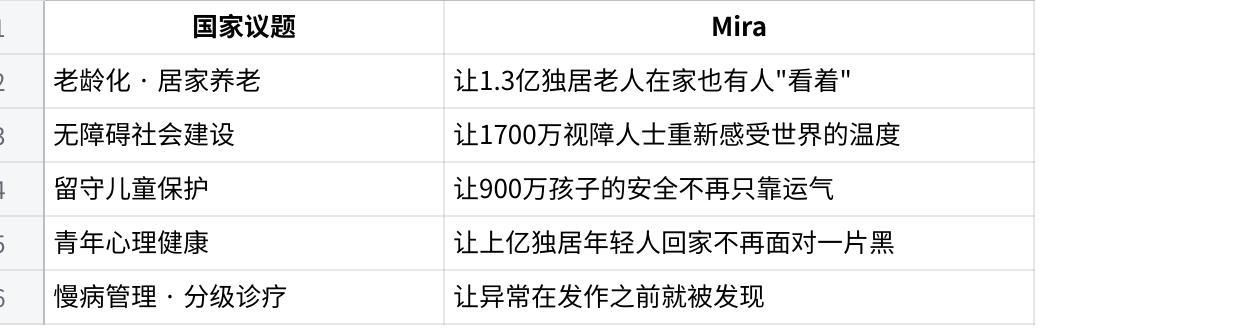
\includegraphics[width=0.94\linewidth]{assets/social-value-table.png}
\end{center}
\vspace{1mm}
{\footnotesize\color{MiraGray}上图整理了项目原始材料中提出的“国家议题—Mira”对应关系：它提醒我们，Mira 的野心并不只是做一个更讨喜的 AI，而是尝试把“被惦记”这件事重新技术化。}

\newpage

% ================= Page 4 =================
\section{Mira 是什么}
\begin{tabularx}{\linewidth}{Y Y}
\begin{accentcard}{一句话定义}
Mira 是一个基于 OpenClaw 的\textbf{主动感受型 AI 伴侣}：它在被授权的设备上接收现实世界信号，在合适时机做判断，并通过\textbf{眼镜、耳机、手表或家居设备}给出尽量小、尽量贴身的回应。
\end{accentcard}
&
\begin{greencard}{一句话气质}
它的理想状态不是“总在说话”，而是\textbf{平时安静、关键时刻出现；知道该做什么，也知道什么时候什么都不做。}
\end{greencard}
\end{tabularx}

\vspace{2mm}
\begin{tabularx}{\linewidth}{L{2.5cm}Y Y}
\rowcolor{MiraSoft}
\textbf{范式} & \textbf{典型交互} & \textbf{局限}\\
\textbf{你找它} & “我有点难过，你陪我聊聊。” & 用户必须先察觉并说出自己的状态\\
\textbf{它找你} & 定时问候、固定频率推送 & 不知道用户此刻究竟发生了什么\\
\textbf{它懂你}（Mira） & \textbf{先观察，再判断，再选择是否行动} & 关键难点转向感知质量、分寸与边界控制\\
\end{tabularx}

\vspace{2mm}
\begin{tabularx}{\linewidth}{Y Y}
\begin{card}{Mira 不是}
\begin{itemize}
  \item 不是全天候喋喋不休的陪聊机器人；
  \item 不是“看到什么都自动执行”的黑盒 agent；
  \item 不是以监控为目的的数据收集系统。
\end{itemize}
\end{card}
&
\begin{card}{Mira 是}
\begin{itemize}
  \item 一个\textbf{把生活信号翻译成照护动作}的 companion system；
  \item 一个强调\textbf{默认沉默、私密输出、最小动作}的陪伴产品；
  \item 一个把\textbf{记忆、感知与执行}放进同一闭环里的现实世界接口。
\end{itemize}
\end{card}
\end{tabularx}

\vspace{2mm}
\begin{goldcard}{产品原则}
\textbf{其一，先判断“值不值得打扰”。} \textbf{其二，优先使用最私密、最轻的通道。} \textbf{其三，动作必须可解释、可限制、可撤销。} 这三条原则，决定了 Mira 与普通自动化 agent 的根本差异。
\end{goldcard}

\newpage

% ================= Page 5 =================
\section{技术原理：从感知到行动}
\begin{center}
\begin{tikzpicture}[node distance=7mm and 7mm,>=Latex]
  \tikzstyle{box}=[rounded corners=4pt, draw=MiraLine, thick, minimum height=16mm, minimum width=34mm, align=center, fill=white]
  \node[box, fill=MiraRose, draw=MiraAccent] (p) {\textbf{Perception}\\眼镜画面\;心率\;环境线索};
  \node[box, right=of p, fill=MiraSoft] (m) {\textbf{Memory}\\短期状态\;长期偏好\;近期事件};
  \node[box, right=of m, fill=MiraBlueSoft, draw=MiraBlue] (j) {\textbf{Judgment}\\是否值得打扰\\动作强度/通道};
  \node[box, right=of j, fill=MiraGreenSoft, draw=MiraGreen] (a) {\textbf{Action}\\镜片提示\;耳机/手表\\家居执行};
  \draw[->, thick, color=MiraAccent] (p) -- (m);
  \draw[->, thick, color=MiraAccent] (m) -- (j);
  \draw[->, thick, color=MiraAccent] (j) -- (a);
\end{tikzpicture}
\end{center}

\vspace{2mm}
\begin{card}{一个足够解释系统行为的简化判定式}
\[
S_t = \alpha V_t + \beta H_t + \gamma C_t + \delta M_t - \lambda R_t
\]
其中，$V_t$ 表示视觉事件显著度，$H_t$ 表示可穿戴侧的生理波动，$C_t$ 表示上下文相关性，$M_t$ 表示记忆检索后的个体匹配程度，$R_t$ 表示动作风险与打扰成本。只有当
\[
S_t > \tau_{\mathrm{act}}\quad \text{且}\quad a_t \in \mathcal{A}_{\mathrm{allow}}
\]
系统才进入行动阶段；否则保持沉默。这一形式并不是为了追求数学花哨，而是为了明确：\textbf{主动感知并不意味着自动出手，Mira 的核心是“先判断，再决定是否行动”。}
\end{card}

\vspace{2mm}
\begin{tabularx}{\linewidth}{Y Y}
\begin{bluecard}{记忆如何发挥作用}
记忆层保存的不是一条条孤立日志，而是\textbf{“这个人最近经历了什么、通常喜欢什么、什么动作曾经被确认过”}。因此同样是心率升高，对一个准备路演的人意味着鼓励，对一个在健身的人则可能什么都不必做。
\end{bluecard}
&
\begin{greencard}{动作如何保持克制}
动作由策略层裁决：\textbf{优先私密、优先轻量、优先可撤销。} 先考虑镜片短句、耳机轻声、手表震动；只有在确有必要时，才进入家庭设备控制或外部通知。
\end{greencard}
\end{tabularx}

\vspace{2mm}
\begin{goldcard}{最简 pipeline}
\texttt{frame + wearable signal + context -> observe -> memory -> policy -> confirm/execute}
\end{goldcard}

\newpage

% ================= Page 6 =================
\section{系统结构与工程落地}
\begin{card}{为什么 Mira 选择 OpenClaw 作为底座}
OpenClaw 官方仓库提供了多通道个人 AI assistant、companion apps、device nodes（包括 camera / screen recording / notifications / location）与 skills/workspace 机制，适合作为 Mira 的\textbf{控制平面与执行容器}；Rokid 开发文档则提供了设备接入与 SDK / 开放平台能力，使眼镜成为可用的现实世界感知前端。需要特别说明的是：\textbf{GitHub 中的文件夹树未来可以重构，但模块逻辑不会变}——无论目录怎么调整，系统本质上仍然由观察入口、记忆层、策略层、确认链路与执行器几部分组成。
\end{card}

\vspace{2mm}
\begin{tabularx}{\linewidth}{L{3.0cm}Y L{2.2cm}}
\rowcolor{MiraSoft}
\textbf{模块} & \textbf{在 Mira 中的职责} & \textbf{当前状态}\\
Rokid bridge / Observe API & 接收来自眼镜或脚本的观察事件，完成标准化输入 & \goodtag{已打通}\\
Gateway / control plane & 负责调度、队列与动作路由，是系统的控制中枢 & \goodtag{已打通}\\
Memory ledger / transient memory & 记录事件、确认、检索上下文，形成可追溯记忆层 & \goodtag{已打通}\\
Policy layer & 评估 quiet hours、风险级别、recipient scope、是否可外发 & \goodtag{已打通}\\
Confirm path & 把中高风险动作放入待确认链路，避免黑盒自动化 & \midtag{部分实现}\\
Home Assistant executor & 将判断翻译成家庭设备动作与生态控制 & \goodtag{已打通}\\
多模态状态融合 & 将视觉、穿戴与记忆一起整合成行动判断 & \midtag{可演示}\\
长期守护型趋势分析 & 面向老人、儿童等长期场景的稳定模型与编排 & \futuretag{路线图}\\
\end{tabularx}

\vspace{2mm}
\begin{tabularx}{\linewidth}{Y Y}
\begin{bluecard}{工程上最重要的改造}
Mira 并没有把 OpenClaw 当作一个“聊天入口”，而是把它当作\textbf{现实世界事件的编排器}：从原来的问答响应，扩展为持续接收观察、检索记忆、做策略评估，并把结果路由到更适合的设备通道。
\end{bluecard}
&
\begin{goldcard}{为什么这条路可复现}
因为它不是纯粹的概念叙事。设备输入、memory ledger、policy 文件、confirm path 与 Home Assistant 执行器都可以拆开验证；也就是说，\textbf{Mira 的核心并不是一句 slogan，而是一条可拆分、可调试、可逐步增强的系统路径。}
\end{goldcard}
\end{tabularx}

\newpage

% ================= Page 7 =================
\section{主 Demo：演讲前主动支持}
\begin{accentcard}{为什么选这个场景}
上台前的紧张，是最容易被忽视、却最适合被技术温柔接住的时刻。用户通常不会在准备登台的最后三十秒专门对 AI 说“我有点慌”，但视觉场景、穿戴信号与近期上下文已经足以构成一条\textbf{高价值、低打扰、可解释}的主动支持闭环。
\end{accentcard}

\vspace{3mm}
\begin{tikzpicture}[node distance=4.6mm and 5mm,>=Latex]
  \tikzset{flowstep/.style={rounded corners=3pt, draw=MiraLine, fill=white, minimum height=11mm, minimum width=24mm, align=center, font=\footnotesize}}
  \node[flowstep, fill=MiraRose, draw=MiraAccent] (s1) {1\\Rokid 识别\\公开表达场景};
  \node[flowstep, right=of s1, fill=MiraSoft] (s2) {2\\心率或体态\\出现紧张信号};
  \node[flowstep, right=of s2, fill=MiraBlueSoft, draw=MiraBlue] (s3) {3\\检索近期准备\\与历史偏好};
  \node[flowstep, right=of s3, fill=MiraGoldSoft, draw=MiraGold] (s4) {4\\策略层判断\\值不值得打扰};
  \node[flowstep, right=of s4, fill=MiraGreenSoft, draw=MiraGreen] (s5) {5\\优先私密通道\\生成最小支持};
  \node[flowstep, right=of s5, fill=MiraSoft] (s6) {6\\镜片/耳机\\输出鼓励};
  \foreach \a/\b in {s1/s2,s2/s3,s3/s4,s4/s5,s5/s6}{\draw[->,thick,color=MiraAccent2] (\a) -- (\b);}
\end{tikzpicture}

\vspace{2mm}
\begin{tabularx}{\linewidth}{Y Y}
\begin{greencard}{示例输出}
“放轻松，你肯定可以做到。先深呼吸。你这两天已经准备得很充分了，去把这个舞台拿下来。”
\end{greencard}
&
\begin{bluecard}{这个 demo 证明了什么}
\begin{itemize}
  \item Mira 的价值不在“更会聊”，而在\textbf{关键时刻少说一句却更有用}；
  \item 系统先做的是\textbf{要不要行动}的判断，而非默认持续输出；
  \item 输出优先落在\textbf{私密界面}，而不是公共暴露或社交外发。
\end{itemize}
\end{bluecard}
\end{tabularx}

\vspace{2mm}
\begin{card}{本阶段建议重点跟踪的三个评估指标}
\textbf{有效触发率}：真正被用户认为“有帮助”的主动触达占比；\quad
\textbf{误打扰率}：本不该触发却触发的比例；\quad
\textbf{闭环时延}：从事件进入到提示落地的总耗时。\par
对陪伴型产品而言，模型分数不是终点，\textbf{分寸感与体感}才是最重要的产品指标。
\end{card}

\newpage

% ================= Page 8 =================
\section{场景扩展与实施边界}
\begin{tabularx}{\linewidth}{Y Y}
\begin{card}{场景 A｜疲惫工作者的回家时刻}
\textbf{输入线索}\;：长时间屏幕注视、全天高压状态、午餐缺失、接近归家时间。\\
\textbf{判断目标}\;：不是去“劝你休息”，而是判断\textbf{是否值得先替你把家变得舒服一点}。\\
\textbf{典型动作}\;：暖色灯光、加湿器、音乐、香薰或温度调节。\\
\textbf{用户感受}\;：它什么都没说，但回家这一刻已经被提前照顾好。
\end{card}
&
\begin{card}{场景 B｜家庭守护与异常提醒}
\textbf{输入线索}\;：久坐不动、步态变化、危险姿态、异常安静、监护对象长期趋势偏移。\\
\textbf{判断目标}\;：把“说不出口的异常”提早变成\textbf{温和而明确的提醒}。\\
\textbf{典型动作}\;：私密通知、家属提醒、询问型消息、待确认动作。\\
\textbf{用户感受}\;：Mira 不是替代家人，而是替家人更早一点注意到风险。
\end{card}
\end{tabularx}

\vspace{2mm}
\begin{tabularx}{\linewidth}{L{2.8cm}Y}
\rowcolor{MiraSoft}
\textbf{能力层级} & \textbf{本次文档中的处理方式}\\
\goodtag{已实现 / 已验证} & Wearable $\rightarrow$ Home Assistant 的动作链路；观察事件进入系统；基础策略层与确认接口；叙事型演讲支持演示。\\
\midtag{部分实现 / 可演示} & 多模态判断拼接、低风险主动提醒、眼镜侧陪伴式输出体验。\\
\futuretag{愿景 / 路线图} & 独居老人趋势守护、儿童长期监护、稳定的社交记忆与更完整的回家照护编排。\\
\end{tabularx}

\vspace{2mm}
\begin{goldcard}{为什么要明确写出“边界”}
因为一个好的项目说明书不应该把所有场景写成同一语气层级。Mira 当前\textbf{已经证明了主动感知和设备执行可以连起来}；更大的守护型场景，是建立在这条主闭环之上的未来扩展，而不是被夸大为已完全交付的现成产品。
\end{goldcard}

\newpage

% ================= Page 9 =================
\section{安全、隐私与社会价值}
\begin{tabularx}{\linewidth}{Y Y}
\begin{accentcard}{主动，不等于越界}
Mira 的难点从来不只是“能不能更早察觉”，而是“能不能在边界内察觉”。如果没有规则约束，主动感知会立刻滑向监控与打扰；因此，\textbf{Mira 的第一产品能力其实是克制。}
\end{accentcard}
&
\begin{greencard}{当前最重要的五条约束}
\begin{itemize}
  \item 默认沉默，不确定不行动；
  \item 中高风险外发动作必须进入确认链路；
  \item 数据处理优先本地，用户拥有暂停与擦除权；
  \item 家居控制只能在 allowlist / whitelist 范围内执行；
  \item 对公共社交外发、秘密数据、原始敏感信息保持严格禁止。
\end{itemize}
\end{greencard}
\end{tabularx}

\vspace{2mm}
\begin{tabularx}{\linewidth}{Y Y Y}
\begin{card}{为什么值得信任}
因为它把\textbf{policy、confirm、allowlist}写进系统，而不是事后靠口头承诺补救。
\end{card}
&
\begin{card}{为什么值得同情它要解决的问题}
因为最需要陪伴的人，恰恰最常把“我没事”说出口。
\end{card}
&
\begin{card}{为什么这件事有社会价值}
它尝试把“有人替你惦记着”变成一种可复制的基础能力，而不只是广告里的温情措辞。
\end{card}
\end{tabularx}

\vspace{3mm}
\begin{center}
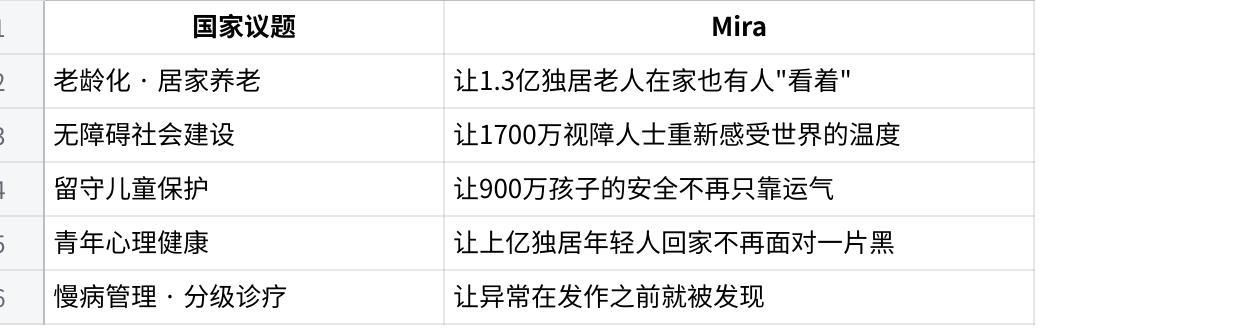
\includegraphics[width=0.94\linewidth]{assets/social-value-table.png}
\end{center}

\vspace{1mm}
\begin{goldcard}{这一页的真正结论}
Mira 追求的不是“更强的监测”，而是\textbf{更有分寸的关怀基础设施}：只在被允许的时候、用被允许的方式、更早一点把帮助送到人身边。
\end{goldcard}

\newpage

% ================= Page 10 =================
\section{路线图、团队与总结}
\begin{tikzpicture}[>=Latex]
  \draw[line width=1.3pt,color=MiraLine] (0,0) -- (\linewidth,0);
  \foreach \x/\title/\body/\col in {
    0.10/Hackathon\ MVP/{演讲前支持、Wearable -> HA、Observe -> Confirm -> Action}/MiraAccent,
    0.48/Next\ 1\ Month/{补强 care policy、日志、确认链路与更稳定的设备执行面}/MiraBlue,
    0.84/3\textendash6\ Months/{扩展到回家关怀、独居守护、长期社交记忆与 companion 发布结构}/MiraGreen}
  {
    \fill[\col] (\x\linewidth,0) circle (2.2pt);
    \node[align=center,anchor=south,font=\bfseries\sffamily\footnotesize\titlecjk,text=\col] at (\x\linewidth,0.18) {\title};
    \node[align=center,anchor=north,text width=0.28\linewidth,font=\footnotesize] at (\x\linewidth,-0.18) {\body};
  }
\end{tikzpicture}

\vspace{24mm}
\begin{tabularx}{\linewidth}{Y Y}
\begin{card}{团队分工}
\textbf{Rick}\par
产品定义、叙事 framing、场景体验、视觉表达与说明书结构。\par\vspace{0.3em}
\textbf{Junkai}\par
后端链路、OpenClaw / Rokid / Home Assistant 接入、安全边界与执行逻辑。
\end{card}
&
\begin{card}{评委最后应记住的三点}
\begin{itemize}
  \item Mira 证明的是\textbf{care loop}，不是更花哨的聊天文案；
  \item 本次比赛已经打通\textbf{主动感知 + 策略判断 + 设备执行}的主路径；
  \item 这套系统的价值，来自\textbf{克制、私密、可控}，而不是“更激进地自动化”。
\end{itemize}
\end{card}
\end{tabularx}

\vspace{2mm}
\begin{accentcard}{总结}
Mira 想证明的不是“AI 可以更炫”，而是：\textbf{AI 可以在合适的时候，更早一点懂你，更稳一点帮你。} 当感知、记忆、判断与执行被放进同一条现实世界闭环里，陪伴才第一次不再只是一句回复，而开始像一种真正发生过的照顾。
\end{accentcard}

\vfill
{\footnotesize\color{MiraGray}资料来源说明：本文档在用户提供的项目说明书、评审 brief、需求文档与展位设计稿基础上重写，并参考 OpenClaw 官方仓库、Rokid 开发文档与 OpenClaw Hackathon 官方活动说明整理而成。}

\end{document}
